\pagebreak 
\centering
\emph{\color{MidnightBlue} \Huge How to find out more about GHRSST:}
\newp
\color{MidnightBlue}{A complete description of GHRSST together with all project documentation can be found at the
following web spaces:}
\par
\begin{longtable}{p{0.3\textwidth} p{0.45\textwidth}}

Main GHRSST portal & https://www.ghrsst.org \\
GHRSST GDAC (rolling archive) & \color{blue}{\url{http://ghrsst.jpl.nasa.gov}} \\
GHRSST LTSRF (Archive) & \color{blue}{\url{http://ghrsst.nodc.noaa.gov}} \\
GHRSST HRDDS (diagnostics) & \color{blue}{\url{http://www.hrdds.net}}\\
GHRSST MDB (validation) & \color{blue}{\url{http://www.ifremer.fr/matchupdb}} \\
GHRSST GMPE (L4 ensembles) &
\color{blue}{\url{http://ghrsst-pp.metoffice.com/pages/latest\_analysis/sst\_monitor/daily/ens/index.html}} \\
GHRSST data discovery & \color{blue}{\url{http://ghrsst.jpl.nasa.gov/data\_search.html}} \\
GHRSST data visualisation (EU) & \color{blue}{\url{http://www.naiad.fr}} \\
GHRSST data visualisation (USA) & \color{blue}{\url{http://podaac-tools.jpl.nasa.gov/dataminer/}} \\
\end{longtable}

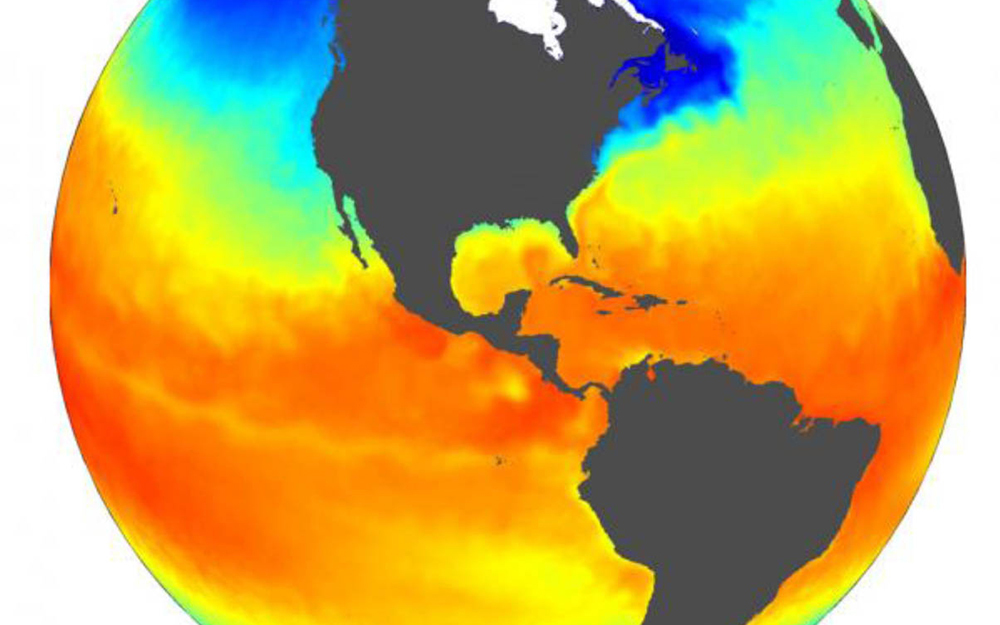
\includegraphics[width=0.4\textwidth]{../images/globe_1000px.jpeg}
\newp

\large{\color{MidnightBlue}\emph{GHRSST International Project Office}} \\
\normalsize
\color{MidnightBlue}NCEO, Department of Meteorology, \\
University of Reading, \\
United Kingdom
\newp

Tel +44 (0) 118 3785579 \\
Fax +44 (0) 118 3785576 \\
E-mail: \\
\color{blue}{ghrsst-po@nceo.ac.uk}
\color{MidnightBlue}

\thispagestyle{empty}
\vfill
\footnotesize The GHRSST International Project Office is sponsored by the European Space Agency
and the National Centre for Earth Observation, United Kingdom.